% ============================================================
%  Cahier des charges fonctionnel -- Application web CIR
%  Complexe Industriel Révélation SARL
%  Compilation : pdflatex (deux passes)
%  Fichiers requis à côté de ce .tex : logo-cir.png, logo-jiuye.png
% ============================================================
\documentclass[11pt,a4paper]{article}

\usepackage[utf8]{inputenc}
\usepackage[T1]{fontenc}
\usepackage[french,provide=*]{babel}
\usepackage[scaled=0.95]{helvet}
\renewcommand{\familydefault}{\sfdefault}

\usepackage[a4paper,top=2.6cm,bottom=2.6cm,left=2.4cm,right=2.4cm,headheight=15pt]{geometry}
\usepackage[table]{xcolor}
\usepackage{graphicx}
\usepackage{tikz}
\usetikzlibrary{positioning,arrows.meta}
\usepackage{tabularx}
\usepackage{array}
\usepackage{enumitem}
\usepackage{titlesec}
\usepackage{fancyhdr}
\usepackage{lastpage}
\usepackage{needspace}
\usepackage[hidelinks]{hyperref}

% ---------- Couleurs tirées du logo CIR ----------
\definecolor{circyan}{HTML}{24C7E6}   % fond du logo
\definecolor{cirblue}{HTML}{1177A8}   % « REVELATION.SARL »
\definecolor{cirgreen}{HTML}{4BA625}  % lettres vertes
\definecolor{circoral}{HTML}{FF6D4C}  % lettres corail
\definecolor{cirgold}{HTML}{9B820C}   % « COMPLEXE INDUSTRIEL »
\definecolor{cirink}{HTML}{1F2D36}    % texte courant
\definecolor{cirtint}{HTML}{EAF8FC}   % cyan très clair (fonds)
\definecolor{cirgrey}{HTML}{6B7880}   % texte secondaire

\color{cirink}
\hypersetup{pdftitle={Cahier des charges fonctionnel -- Application web CIR},
            pdfauthor={Complexe Industriel Révélation SARL}}

% ---------- Mise en forme générale ----------
\setlength{\parindent}{0pt}
\setlength{\parskip}{0.7em}
\linespread{1.08}
\setlist[itemize]{leftmargin=1.4em,itemsep=0.25em,topsep=0.3em,
                  label={\color{circoral}\rule[0.25ex]{0.45em}{0.45em}}}

% ---------- Titres ----------
\titleformat{\section}
  {\Large\bfseries\color{cirblue}}
  {\color{circoral}\thesection}{0.7em}{}
  [{\color{circyan}\titlerule[1.4pt]}]
\titlespacing*{\section}{0pt}{1.8em}{0.9em}
\titleformat{\subsection}
  {\large\bfseries\color{cirblue}}
  {\color{circoral}\thesubsection}{0.6em}{}
\titlespacing*{\subsection}{0pt}{1.15em}{0.3em}
\titleformat{\subsubsection}
  {\normalsize\bfseries\color{cirgold}}
  {}{0pt}{}
\titlespacing*{\subsubsection}{0pt}{1.1em}{0.2em}

% ---------- En-tête et pied de page ----------
\pagestyle{fancy}
\fancyhf{}
\fancyhead[L]{\footnotesize\color{cirgrey}Cahier des charges fonctionnel --- Application web CIR}
\fancyhead[R]{\footnotesize\color{cirgrey}Complexe Industriel Révélation SARL}
\fancyfoot[C]{\footnotesize\color{cirgrey}Page \thepage\ sur \pageref{LastPage}}
\renewcommand{\headrulewidth}{0.8pt}
\renewcommand{\headrule}{{\color{circyan}\hrule height \headrulewidth}}

% ---------- Outils ----------
% Astérisque : élément ajouté en complément de la dictée
\newcommand{\prop}{\textsuperscript{\color{circoral}\textbf{*}}}

% Bande tricolore reprenant les couleurs du logo
\newcommand{\bandecir}[1][1.2cm]{%
  {\color{cirgreen}\rule{#1}{3pt}}{\color{circoral}\rule{#1}{3pt}}{\color{cirblue}\rule{#1}{3pt}}}

% Encadré de mise en avant
\newcommand{\encadre}[2]{%
  \par\smallskip\noindent
  {\color{circoral}\vrule width 3pt}%
  \colorbox{cirtint}{\parbox{\dimexpr\linewidth-3pt-2\fboxsep\relax}{%
    \vspace{0.3em}\hspace{0.4em}\textbf{\color{cirblue}#1}\par\vspace{0.15em}
    \leftskip=0.4em \rightskip=0.4em #2\par\vspace{0.3em}}}%
  \par\smallskip}

% Tableaux de besoins : Réf. | Intitulé | Description
\renewcommand{\arraystretch}{1.45}
\newcolumntype{R}{>{\leavevmode\bfseries\color{cirblue}}p{1.55cm}}
\newcolumntype{T}{>{\raggedright\arraybackslash\bfseries}p{3.7cm}}
\newcolumntype{Y}{>{\raggedright\arraybackslash}X}
\newcommand{\entete}[3]{%
  \rowcolor{cirblue}\multicolumn{1}{l}{\color{white}\bfseries #1} &
  \multicolumn{1}{l}{\color{white}\bfseries #2} &
  \multicolumn{1}{l}{\color{white}\bfseries #3}\\}
\newenvironment{besoins}
  {\rowcolors{2}{white}{cirtint}\tabularx{\linewidth}{R T Y}%
   \entete{Réf.}{Besoin}{Description}}
  {\endtabularx\rowcolors{2}{}{}}

% ============================================================
\begin{document}

% ---------------------- Page de garde ----------------------
\begin{titlepage}
\begin{tikzpicture}[remember picture,overlay]
  % bandeau cyan : même teinte que le fond du logo
  \fill[circyan] (current page.north west) rectangle
        ([yshift=-11.2cm]current page.north east);
  \IfFileExists{logo-cir.png}{%
    \node[anchor=north] at ([yshift=-1.3cm]current page.north)
          {\includegraphics[width=8.6cm]{logo-cir.png}};}{}
  % liseré tricolore sous le bandeau
  \fill[cirgreen] ([yshift=-11.2cm]current page.north west) rectangle
        ([xshift=7cm,yshift=-11.38cm]current page.north west);
  \fill[circoral] ([xshift=7cm,yshift=-11.2cm]current page.north west) rectangle
        ([xshift=14cm,yshift=-11.38cm]current page.north west);
  \fill[cirblue] ([xshift=14cm,yshift=-11.2cm]current page.north west) rectangle
        ([yshift=-11.38cm]current page.north east);
\end{tikzpicture}

\vspace*{10.4cm}

{\color{cirgold}\bfseries\large CAHIER DES CHARGES FONCTIONNEL\par}
\vspace{0.6cm}
{\color{cirblue}\bfseries\fontsize{30}{36}\selectfont Application web CIR\par}
\vspace{0.5cm}
{\Large\color{cirink} Vitrine, catalogue et prise de commande\\[0.2em]
 pour les revêtements de sol en résine époxy\par}

\vfill

\bandecir\par\vspace{0.5cm}
{\large\bfseries\color{cirblue} Complexe Industriel Révélation SARL\par}
\vspace{0.2cm}
{\color{cirgrey} Version 1.2 \quad|\quad Octobre 2026\par}

\IfFileExists{logo-jiuye.png}{%
\begin{tikzpicture}[remember picture,overlay]
  \node[anchor=south east,align=center,inner sep=0pt]
        at ([xshift=-2.4cm,yshift=2.6cm]current page.south east)
        {{\footnotesize\color{cirgrey} Entreprise partenaire}\\[0.35cm]
         \includegraphics[height=3.1cm]{logo-jiuye.png}};
\end{tikzpicture}}{}
\end{titlepage}

% ---------------------- Sommaire ----------------------
\tableofcontents
\vspace{1.5em}
\encadre{Lecture du document}{Les éléments marqués d'un astérisque~\prop{} ne
figurent pas dans les indications d'origine~: ce sont des compléments proposés,
à valider ou à retirer.}
\newpage

% ============================================================
\section{Présentation du projet}

\subsection{Contexte}

Dans son contexte social et économique, l'Afrique centrale est soumise à
certaines limites technologiques et industrielles. Il en résulte l'utilisation
et la conservation de méthodes parfois dépassées, notamment dans le domaine du
revêtement des sols.

Pour des raisons économiques, voire écologiques, les populations sont souvent
contraintes de s'en tenir à des solutions classiques~: l'on voit encore des
sols revêtus de ciment, parfois de carreaux, qui posent des problèmes de
résistance et de durabilité.

\subsection{L'entreprise et son offre}

Au vu de cette situation industrielle locale, le \textbf{Complexe Industriel
Révélation SARL} (CIR) met à la disposition de l'Afrique centrale une touche de
nouveauté~: une peinture en résine époxy qui offre

\begin{itemize}
  \item un revêtement de sol \textbf{durable}~;
  \item une décoration \textbf{unique}~;
  \item un \textbf{coût} qui bat la concurrence.
\end{itemize}

\begin{minipage}[c]{0.88\linewidth}
Installé à Douala (Cameroun), le CIR s'appuie sur une entreprise partenaire~:
\textbf{Jiuye} (Guangdong Jiuye New Materials Co., Ltd.), fabricant chinois de
revêtements de sol fondé en 2006, dont le catalogue présente le CIR comme
son distributeur en Afrique centrale.
\end{minipage}\hfill
\begin{minipage}[c]{0.09\linewidth}\centering
\IfFileExists{logo-jiuye.png}{\includegraphics[height=1.75cm]{logo-jiuye.png}}{}
\end{minipage}

\subsection{L'application web CIR}

C'est dans ce cadre qu'intervient l'application web CIR. Elle démontrera à
l'ensemble de ses visiteurs la beauté, la qualité et la touche unique
qu'apporte cette peinture en résine époxy, tout en leur permettant de passer
des commandes et de négocier le revêtement de leur maison, de leur industrie
ou de leur entreprise.

\subsection{Objectifs}
\enlargethispage{\baselineskip}% garde les cinq objectifs sur la même page

\begin{enumerate}[label={\color{circoral}\bfseries O\arabic*.},leftmargin=2.4em,itemsep=0.4em]
  \item \textbf{Permettre la commande en ligne.} Les utilisateurs consultent
        les designs qui leur conviennent, sollicitent l'équipe pour obtenir un
        design particulier et concluent des contrats pour le revêtement de
        leurs maisons, de leurs industries ou de leurs entreprises.
  \item \textbf{Mettre en avant le produit.} L'application valorise la qualité
        et la beauté du résultat obtenu avec la peinture en résine époxy.
  \item \textbf{Informer en continu.} Les utilisateurs ne manquent aucune
        nouveauté et découvrent également les autres produits du Complexe
        Industriel Révélation SARL.
  \item \textbf{Inspirer confiance.}\prop{} Les réalisations, les
        démonstrations, les témoignages de clients et le partenariat avec le
        fabricant Jiuye apportent la preuve concrète de la qualité annoncée.
  \item \textbf{Faciliter la gestion interne.}\prop{} L'équipe du CIR dispose
        d'un outil unique pour tenir à jour le catalogue et traiter les
        commandes et les demandes.
\end{enumerate}

% ============================================================
\Needspace{14\baselineskip}
\section{Catalogue de référence}
\label{sec:catalogue}

Le contenu de l'application s'appuie sur le catalogue transmis par le CIR~: la
brochure en français de la marque Jiuye (24~doubles pages). Elle fournit la
matière du catalogue en ligne (BF-01), des détails techniques (BF-06) et, en
partie, des réalisations (BF-02).

\subsection{Familles de produits}
\label{sec:familles}

Le catalogue compte une trentaine de références, réparties en neuf familles.

\begingroup
\rowcolors{2}{white}{cirtint}
\begin{tabularx}{\linewidth}{>{\leavevmode\bfseries\color{cirblue}\raggedright\arraybackslash}p{3.5cm} >{\raggedright\arraybackslash}p{4.2cm} Y}
  \entete{Famille}{Références}{Usages}
  Primaires époxy & YD-103, YD-104, YD-30\# &
    Préparation du support en béton, ancien ou neuf.\\
  Couche intermédiaire époxy & YD-205 &
    Mortier intermédiaire, coloré ou incolore.\\
  Finitions & YD-148, YD-143, YD-140, YD-500, YD-306, YD-518, YD-147,
    YD-650F, YD-908, YD-909, YD-315, YD-508 &
    Finition lisse, mate ou antidérapante, sol autolissant, sable coloré,
    terrazzo, anti-UV, anticorrosion, haute résistance à l'usure,
    antistatique.\\
  Époxy sans solvant & YD-106W, YD-206W, YD-306W &
    Primaire, couche intermédiaire et finition sans solvant.\\
  Gamme à base d'eau & YD-101S, YD-202S, YD-303S, YD-803, YD-601, YD-ECC,
    YD-8210, YD-8280 &
    Époxy et polyuréthane à l'eau, pour les lieux à exigences
    environnementales (santé, alimentaire, écoles, habitat).\\
  Peintures de marquage & YD-901, YD-1488, YD-301 &
    Traçage des routes, des parkings et des ateliers.\\
  Traitement du béton & --- &
    Durcisseur et scellant, colorant, brillanteur.\\
  Sols spéciaux & --- &
    Sol perméable d'extérieur, terrains de sport, piste d'athlétisme.\\
  Produits complémentaires & YD-501, YD-502 &
    Primaire antirouille, peinture pour tuiles, mastic pour joints,
    aménagement et signalisation de parking.\\
\end{tabularx}
\endgroup

\encadre{Recommandation\prop}{Le catalogue est surtout tourné vers
l'industrie. Pour l'habitat et la décoration, mis en avant dans les objectifs,
les gammes les plus parlantes sont le sol autolissant (YD-500), le sable coloré
(YD-306) et le terrazzo époxy (YD-518)~: elles gagneraient à ouvrir le
catalogue en ligne.}

\Needspace{10\baselineskip}
\subsection{Structure d'une fiche produit}
\label{sec:fiche}

Chaque fiche du catalogue suit la même trame, à reprendre pour la page produit
de l'application~:

\begin{itemize}
  \item référence, nom du produit et photo~;
  \item présentation et domaine d'application~;
  \item caractéristiques de performance~;
  \item mise en œuvre~: préparation, méthode d'application, dosage au m²,
        conditions de chantier~;
  \item plan de coupe montrant les couches du revêtement~;
  \item tableau des indicateurs techniques (temps de séchage, adhérence,
        etc.).
\end{itemize}

\subsection{Réalisations présentées}

Le catalogue montre des chantiers types du fabricant (parkings, bâtiments
industriels, écoles, établissements de santé), tous situés en Chine. Ils
peuvent illustrer les usages, mais ne remplacent pas les chantiers réalisés
par le CIR, attendus pour les réalisations (BF-02), les démonstrations (BF-03)
et les témoignages (BF-04).

\encadre{Coordonnées figurant au catalogue}{Localisation~: Total Nkolmbong,
Douala. Contact~: (00237)~678\,829\,313. WhatsApp~: (00237)~622\,191\,931 et
(00237)~699\,811\,635.}

% ============================================================
\Needspace{9\baselineskip}
\section{Acteurs de l'application}

\begingroup
\rowcolors{2}{white}{cirtint}
\begin{tabularx}{\linewidth}{>{\leavevmode\bfseries\color{cirblue}}p{3.2cm} Y}
  \rowcolor{cirblue}\multicolumn{1}{l}{\color{white}\bfseries Acteur} &
  \multicolumn{1}{l}{\color{white}\bfseries Rôle}\\
  Visiteur & Toute personne qui consulte l'application sans compte~: elle
             découvre les produits, les réalisations, les prix et les
             nouveautés.\\
  Client & Utilisateur inscrit ayant renseigné son adresse. Il peut
           sélectionner des designs, passer commande et négocier son projet
           avec l'équipe.\\
  Administrateur & Membre de l'équipe du CIR. Il gère la plateforme depuis un
           tableau de bord d'administration distinct du site public.\\
\end{tabularx}
\endgroup

% ============================================================
\Needspace{14\baselineskip}
\section{Spécification des besoins}

\subsection{Besoins fonctionnels}

\Needspace{10\baselineskip}
\subsubsection{Découverte des produits (visiteur et client)}

\begin{besoins}
  BF-01 & Catalogue des produits &
    Consulter les produits et les designs de revêtement proposés par le CIR,
    présentés en images et classés par famille (section~\ref{sec:familles}).\\
  BF-02 & Réalisations &
    Voir le résultat de la peinture en action sur des chantiers déjà
    réalisés.\\
  BF-03 & Démonstrations &
    Visionner de courtes démos, notamment chez des clients où la peinture a
    été appliquée.\\
  BF-04 & Témoignages &
    Consulter les témoignages des clients.\\
  BF-05 & Prix &
    Voir les prix fixés pour certains produits.\\
  BF-06 & Détails techniques &
    Connaître précisément l'apport du produit en matière de durabilité, de
    beauté et de confort, selon la trame de fiche de la
    section~\ref{sec:fiche}.\\
  BF-07 & Nouveautés &
    Ne manquer aucune nouveauté ni aucun des différents produits de
    l'entreprise.\\
\end{besoins}

\Needspace{10\baselineskip}
\subsubsection{Commande et échange avec l'équipe}

\begin{besoins}
  BF-08 & Inscription et connexion &
    Créer un compte, renseigner son adresse et se connecter.\\
  BF-09 & Sélection de catalogues &
    Sélectionner un ou plusieurs catalogues ou designs en particulier.\\
  BF-10 & Passage de commande &
    Passer commande à partir de sa sélection, pour une maison, une industrie
    ou une entreprise.\\
  BF-11 & Contact et design sur mesure &
    Contacter l'équipe et discuter avec elle pour obtenir un rendu
    particulier.\\
  BF-12 & Négociation &
    Négocier le revêtement de son bâtiment avec l'équipe, jusqu'à la
    conclusion d'un contrat.\\
  BF-13\prop & Suivi de commande &
    Consulter l'état d'avancement de ses commandes et de ses demandes.\\
\end{besoins}

\encadre{Règle de gestion}{Un utilisateur ne peut passer une commande qu'après
s'être inscrit et avoir donné son adresse.}

\Needspace{10\baselineskip}
\subsubsection{Administration de la plateforme}

\begin{besoins}
  BF-14\prop & Gestion du catalogue &
    Ajouter, modifier et retirer les produits, les designs, les prix et les
    fiches techniques.\\
  BF-15\prop & Gestion des contenus &
    Publier les réalisations, les démos, les témoignages et les nouveautés.\\
  BF-16\prop & Gestion des commandes &
    Consulter et traiter les commandes, répondre aux demandes de design
    particulier et aux négociations.\\
  BF-17\prop & Gestion des utilisateurs &
    Consulter les comptes clients et gérer les accès des administrateurs.\\
\end{besoins}

\Needspace{12\baselineskip}
\subsection{Besoins non fonctionnels}

\begin{besoins}
  BNF-01 & Sécurité &
    L'application protège l'identité et les données personnelles des
    utilisateurs. La commande est réservée aux utilisateurs inscrits ayant
    renseigné leur adresse.\\
  BNF-02 & Performance &
    Chaque page se charge en 3~secondes au plus.\\
  BNF-03 & Ergonomie et fluidité &
    La navigation est très fluide, simple et sans temps mort entre les
    écrans.\\
  BNF-04\prop & Adaptation aux écrans &
    L'application s'affiche correctement sur téléphone, tablette et
    ordinateur.\\
  BNF-05\prop & Images optimisées &
    Le catalogue étant riche en images, celles-ci sont compressées et chargées
    progressivement afin de rester utilisables avec une connexion lente.\\
  BNF-06\prop & Protection technique &
    Les échanges sont chiffrés (HTTPS) et les mots de passe ne sont jamais
    stockés en clair.\\
  BNF-07\prop & Compatibilité &
    L'application fonctionne sur les versions récentes de Chrome, Firefox,
    Safari et Edge.\\
  BNF-08\prop & Disponibilité et sauvegarde &
    L'application reste accessible en continu et ses données sont
    sauvegardées régulièrement.\\
  BNF-09\prop & Maintenabilité &
    Le code est organisé et documenté~; l'ajout d'un produit ou d'un contenu
    ne demande aucun développement.\\
  BNF-10\prop & Référencement &
    Les pages publiques sont conçues pour être bien indexées par les moteurs
    de recherche.\\
\end{besoins}

% ============================================================
\newpage
\section{Spécifications techniques}

\subsection{Choix technologiques}

\begingroup
\rowcolors{2}{white}{cirtint}
\begin{tabularx}{\linewidth}{>{\leavevmode\bfseries\color{cirblue}}p{3.4cm} >{\raggedright\arraybackslash\bfseries}p{3.9cm} Y}
  \entete{Composant}{Technologie}{Rôle}
  Front-end & React &
    Interface du site public~: catalogue, réalisations, compte client,
    commande.\\
  Back-end & Django &
    Logique de l'application~: comptes, catalogue, commandes, échanges avec
    l'équipe.\\
  Administration & Tableau de bord à part &
    Application distincte de la plateforme publique, réservée à l'équipe du
    CIR.\\
  API\prop & Django REST Framework &
    Échanges de données entre les interfaces et le back-end (REST, JSON).\\
  Base de données\prop & PostgreSQL &
    Stockage des utilisateurs, des produits, des commandes et des contenus.\\
  Authentification\prop & Jetons (JWT) &
    Connexion sécurisée des clients et des administrateurs.\\
  Hébergement\prop & À définir &
    Serveur, nom de domaine et stockage des images.\\
\end{tabularx}
\endgroup

\Needspace{14\baselineskip}
\subsection{Architecture générale}

\begin{center}
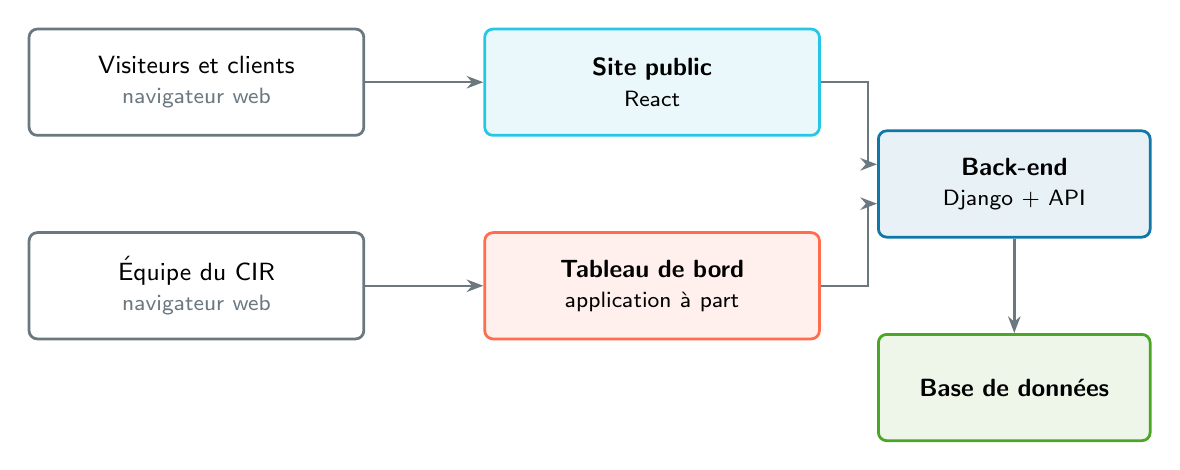
\begin{tikzpicture}[
    font=\small,
    boite/.style={draw=#1,line width=1pt,rounded corners=3pt,
                  minimum height=1.35cm,text width=3.9cm,align=center,
                  inner sep=5pt},
    fleche/.style={-{Stealth[length=6pt]},line width=0.9pt,color=cirgrey},
    node distance=1.2cm and 1.5cm]
  \node[boite=cirgrey] (util) {Visiteurs et clients\\{\footnotesize\color{cirgrey}navigateur web}};
  \node[boite=circyan,fill=cirtint,right=of util] (front)
        {\textbf{Site public}\\{\footnotesize React}};
  \node[boite=cirgrey,below=of util] (equipe) {Équipe du CIR\\{\footnotesize\color{cirgrey}navigateur web}};
  \node[boite=circoral,fill=circoral!10,right=of equipe] (admin)
        {\textbf{Tableau de bord}\\{\footnotesize application à part}};
  \path (front) -- (admin) coordinate[midway] (mil);
  \node[boite=cirblue,fill=cirblue!10,right=4.6cm of mil,anchor=center,text width=3.1cm] (back)
        {\textbf{Back-end}\\{\footnotesize Django + API}};
  \node[boite=cirgreen,fill=cirgreen!10,below=of back,text width=3.1cm] (bdd)
        {\textbf{Base de données}};
  \draw[fleche] (util) -- (front);
  \draw[fleche] (equipe) -- (admin);
  \draw[fleche] (front.east) -- ++(0.6,0) |- ([yshift=0.25cm]back.west);
  \draw[fleche] (admin.east) -- ++(0.6,0) |- ([yshift=-0.25cm]back.west);
  \draw[fleche] (back) -- (bdd);
\end{tikzpicture}
\end{center}

\subsection{Espace d'administration}

La plateforme publique et le tableau de bord d'administration sont deux
applications séparées. Le tableau de bord n'est pas visible depuis le site
public~: il est accessible par une adresse distincte et réservé aux membres
autorisés de l'équipe du CIR, après authentification. Les deux applications
partagent le même back-end Django et la même base de données.

% ============================================================
\Needspace{10\baselineskip}
\section{Points à préciser}

\begin{itemize}
  \item \textbf{Produits commercialisés.} Le CIR propose-t-il toute la gamme
        du catalogue, ou seulement une sélection~? Laquelle~?
  \item \textbf{Prix.} Le catalogue n'en contient aucun. Les prix à afficher
        (BF-05) sont à fournir, avec leur unité~: au m², au kilogramme, pose
        comprise ou non.
  \item \textbf{Réalisations locales.} Photos, démos et témoignages des
        chantiers du CIR restent à transmettre.
  \item \textbf{Partenaire Jiuye.} Le site affiche-t-il le logo et une
        présentation de Jiuye, ou la marque CIR seule~? L'accord du partenaire
        pour reprendre son logo et les images de son catalogue est à
        confirmer.
  \item \textbf{Textes du catalogue.} La traduction française est
        approximative et devra être réécrite. Certaines références diffèrent
        entre le sommaire et les fiches (YD-304W et YD-306W~; YD-701S, 702S,
        704S et YD-101S, 202S, 303S)~: ce document suit les fiches.
  \item \textbf{Délai de chargement.} L'indication d'origine mentionne
        3~millisecondes~; la valeur retenue ici est de 3~secondes, objectif
        réaliste pour une page web. À confirmer.
  \item \textbf{Paiement.} La commande donne-t-elle lieu à un paiement en
        ligne (carte, mobile money), ou le règlement se fait-il hors
        application, à la signature du contrat~?
  \item \textbf{Discussion avec l'équipe.} Messagerie intégrée à
        l'application, formulaire de contact, ou renvoi vers les numéros
        WhatsApp du catalogue~?
  \item \textbf{Nouveautés.} Affichage sur le site uniquement, ou
        notifications par e-mail ou SMS~?
  \item \textbf{Langues.} Français seul, ou français et anglais~?
\end{itemize}

\end{document}
